\section{Baseline Design Validation and Projected Photon Detector Performance}
\label{sec:dp-pds-performance}

After the initial simulation studies described in the \dshort{tp} \cite{Abi:2018rgm}, we have progressed toward a more realistic understanding of the projected \dshort{pds} performance using the \dshort{larsoft} framework:
%
\begin{itemize}
\item Optical simulations are now performed in the \dword{dp} \dword{fd} module geometry. In the \dword{fd} \dshort{tp}, physics studies assumed the \dword{pddp} geometry. Considering the lack of any optical segmentation in the \dword{dp} design, light is simulated in the full \dpactivelarmass \dshort{tpc} active volume. Simulation assumptions for light generation and light transport are described in Section~\ref{subsec:dp-pds-simulation_assumptions}. For each of the \dpnumpmtch \dwords{pmt}, simulations take into account how the photon detection probabilities and the photon propagation times vary throughout the \dshort{tpc} active volume.
%
\item The electronics response and the reconstruction of optical hits and optical clusters has been simulated. Simulation assumptions for light detection by the \dwords{pmt} are also described in Section~\ref{subsec:dp-pds-simulation_assumptions}. Optical hits are the reconstructed optical signals on single \dshort{pmt} waveforms and are characterized by a hit time, amplitude, and charge. Optical hits must have an amplitude of at least \SI{10}{ADC counts} above baseline. Optical clusters refer to a collection of \dshort{pmt} hits correlated in time and space. They are typically induced by the same underlying flash of scintillation light in \lar. The parameters of the clustering algorithm are discussed later in this section.

%
\item The physics studies now also include radiological backgrounds. Simulating radiological backgrounds is critical in realistically optimizing the optical reconstruction parameters. The radiological model includes several radio-isotopes throughout the \lar volume, with \SI{1.01}{\becquerel/\kg} of $^{39}$Ar providing the most activity. In addition, an impinging neutron flux of \SI{e-5}{\cm$^{-2}$\s$^{-1}$} is accounted for.
\end{itemize} 

Expected \dword{pds} light yields in the \dword{pddp} and \dword{dp} \dword{fd} module geometries are discussed in Section~\ref{subsec:dp-pds-simulation_yields}

%%%%%%%%%%%%%%%%%%%%%%%%%%%%%%%%%%%%%%%%%%%%%%%%%%%%%%%%%%%%%%%%%%%%

\subsection{Event $t_{0}$ Reconstruction}
\label{subsec:dp-pds-performance_t0}

As discussed in Section~\ref{sec:dp-pds-requirements}, event $t_0$ reconstruction for non-beam events via the \dshort{pds} is particularly important to fiducialize nucleon decay candidates in \dword{dune}. Proton decay signal events with a %\ptoknubar 
$p\rightarrow K^{+} \bar\nu$ final state have been simulated with GENIE \cite{Andreopoulos:2009rq} throughout the \dword{dp} \dshort{tpc} active volume, and their optical clusters were reconstructed using the full simulation and reconstruction chain. \dword{ndk} events should deposit approximately \SI{400}{\MeV} visible energy in the \lar. The same reconstruction algorithm has also been applied to the simulated radiological backgrounds. In a first cluster reconstruction step, three parameters are optimized to group optical hits into separate clusters:
%
\begin{description}
\item[Maximum cluster duration:] maximum time difference among all \dshort{pmt} hits in the cluster.
\item[Maximum hit time distance:] maximum time difference between successive \dshort{pmt} hits in the cluster. By definition, this quantity is smaller than, or equal to, the maximum cluster duration.
\item[Maximum hit distance:] maximum spatial distance between neighbouring \dshort{pmt} hits in the cluster. 
\end{description}

For each chosen set of parameters (maximum cluster duration, maximum hit time distance, maximum hit distance), a threshold for minimum cluster charge (in \dwords{pe}) is defined, so a fixed, and tolerable, radiological background rate above threshold and per \SI{8}{\milli\s} maximum drift time is obtained. The chosen parameters are those that maximize the efficiency of detecting a \dword{ndk} cluster higher than this minimum cluster charge. For the \dword{pds} baseline design with half foils, the optimal values for the maximum cluster duration, maximum hit time distance and maximum hit distance were found to be \SI{100}{\ns}, \SI{100}{\ns} and \SI{5.5}{\m}, respectively. In other words, optical hits belonging to the same cluster are required to be nearly coincident in time, but only loosely correlated in space. As expected, it was also found that this optimization process yields a different result for a no foil \dword{pds} configuration, where light is more concentrated in space. 

After clustering optical hits as described above, and without applying any threshold on cluster charge, several optical clusters per event are reconstructed. At this stage, any deposit resulting in at least one optical hit is reconstructed by the \dshort{pds}, giving negligible \dword{ndk} optical cluster inefficiency but very high radiological background cluster multiplicity per event. 

In a second optimization step, we define the $t_0$ candidate clusters in the event as the ones fulfilling one additional condition: {\bf cluster spatial position}.

Albeit much less accurate than the \dshort{tpc} response, the \dshort{pds} response also provides some spatial information about the event in the plane perpendicular to the drift direction. The position of the $t_0$ candidate cluster in the plane perpendicular to the drift must be within \SI{1.5}{\m} of the simulated \dword{ndk} decay vertex\footnote{The matching in position with the MC truth information is of course only possible in simulations. However, we expect the \dshort{tpc} imaging performance to be so superior to the \dshort{pds} one that matching \dshort{pds} position with MC truth position is essentially equivalent to matching \dshort{pds} position with \dshort{tpc} reconstructed position.}. Because radiological clusters are randomly distributed with respect to the \dword{ndk} vertex, this position matching provides a strong background cluster suppression of about two orders of magnitude.

We define the {\bf \dword{ndk} $t_0$ reconstruction efficiency} as the efficiency to reconstruct at least one $t_0$ candidate cluster associated to the \dword{ndk} energy deposit. As shown below, the cluster spatial position requirement causes some inefficiency for events farther from the \dshort{pds} because of poorly reconstructed cluster spatial position in the plane perpendicular to the drift.

In general, several $t_0$ candidate clusters will be reconstructed per event, induced by the \dword{ndk} signal, by radiological activity, and by \dshort{pmt} dark counts. If more than one choice exists, event $t_0$ information is associated to the $t_0$ candidate cluster of highest charge. For events where at least one $t_0$ candidate cluster exists, we define the {\bf \dword{ndk} $t_0$ reconstruction purity} as the probability for the highest charge $t_0$ candidate cluster in the event to be associated with the \dword{ndk} signal. A purity value $<1$ can be obtained if the highest charge $t_0$ candidate cluster is due to radiological activity. The choice of the $t_0$ candidate cluster with the highest charge is made to maximize purity because radiological clusters have, on average, fewer reconstructed \dwords{pe} per cluster. As discussed in Section~\ref{sec:dp-pds-requirements}, we require a high purity to minimize $t_0$ reconstruction ambiguities.
%

\begin{dunefigure}[Optimization of $t_0$ candidate cluster spatial position reconstruction for \dword{ndk} events.]{fig:dppd_ndk_optimization}
{Efficiency, purity, and efficiency times purity for the $t_0$ candidate cluster to be correctly associated to the \dword{ndk} energy deposit, as a function of the maximum 2D distance between the \dshort{pds}-reconstructed position of the $t_0$ candidate cluster and the actual \dword{ndk} vertex, in the plane perpendicular to drift. A maximum distance of \SI{1.5}{\m} optimizes the product of efficiency times purity.}
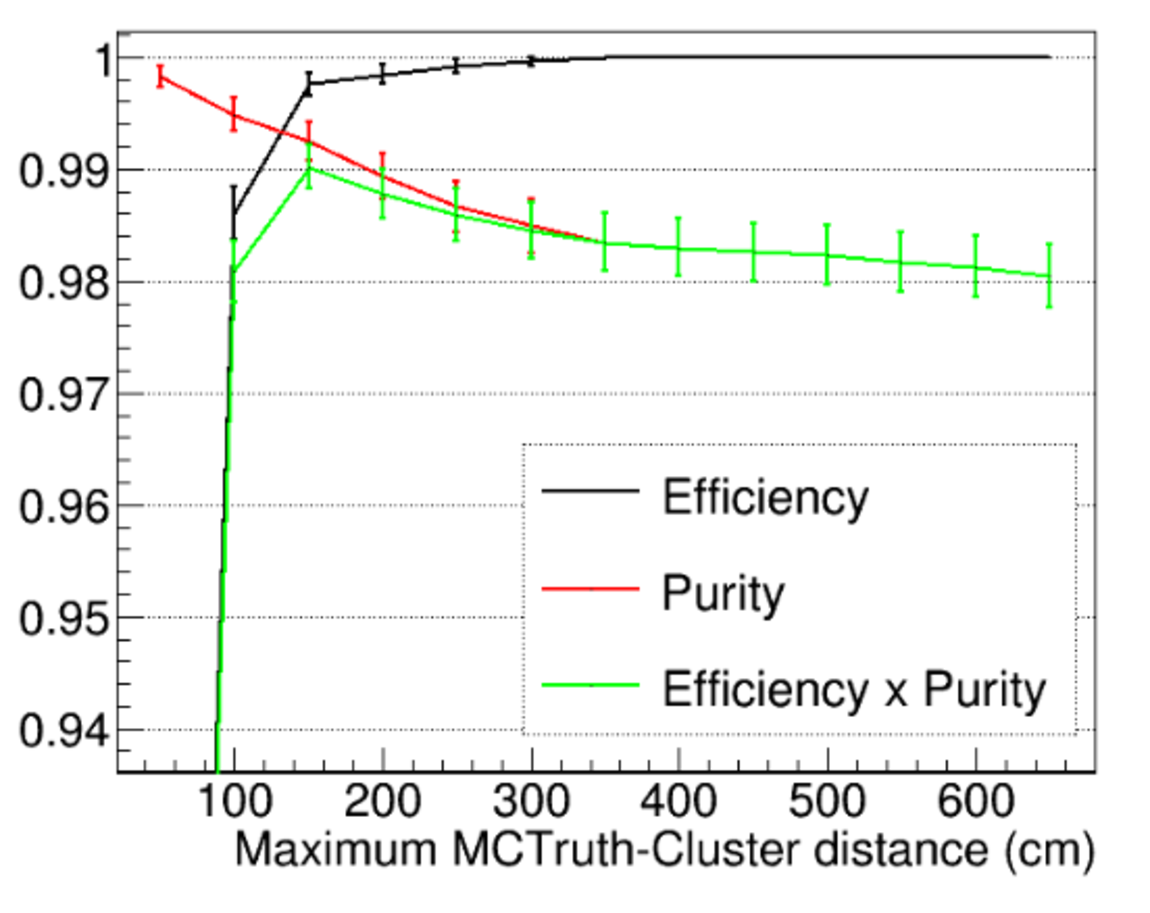
\includegraphics[width=0.5\textwidth]{graphics/dppd_ndk_optimization.pdf}
\end{dunefigure}

Figure~\ref{fig:dppd_ndk_optimization} illustrates how the \dword{ndk} signal efficiency, purity, and efficiency$\times$purity averaged over the entire \dshort{tpc} active volume vary as a function of the maximum 2D distance between the $t_0$ candidate cluster reconstructed position and the \dword{ndk} vertex actual position in the plane perpendicular to drift. A maximum distance of \SI{1.5}{\m} optimizes the product of efficiency$\times$purity. For this optimal distance, an average efficiency value of \num{99.8}\% and purity value of \num{99.2}\% are obtained.  

Figure~\ref{fig:dppd_ndk_efficiency} shows how the \dword{ndk} $t_0$ reconstruction efficiency and purity vary as a function of the nucleon decay vertex distance from the cathode plane for the optimal cluster reconstruction parameters described above. Two configurations are compared: the proposed baseline design with half foils, and a design with no foils along the \dword{fc}. For the baseline design, both the efficiency and purity remain $>90\%$ throughout the \dword{tpc} active volume, satisfying the detector requirements laid out in Sec.~\ref{subsec:dp-pds-requirements_requirements}. From Figure~\ref{fig:dppd_fd_light_yield_comparisons}, a light yield of \SI{1}{PE/\MeV} is expected at the anode plane in the half foil simulation. Because of this, the \dword{pds} minimum light yield required at the anode position is also \SI{1}{PE/\MeV} (see Table~\ref{tab:specs:just:DP-PDS}). 

On the other hand, for the no foil configuration, both efficiency and purity drop rapidly at large distances from the cathode. This is due to the marked reduction in the detected \dword{ndk} light yield as the energy deposition occurs at increasingly larger distances from the cathode, see Figure~\ref{fig:dppd_fd_light_yield_comparisons}. In this case, the efficiency (purity) remains $>90\%$ only for distances up to \SI{10}{\m} (\SI{7}{\m}) from the cathode. This large improvement in efficiently and accurately reconstructing event $t_0$ information for \dword{ndk} events is the main, but not only, motivation to introduce reflector/\dword{wls} foils along the \dword{fc} walls in the baseline design.

\begin{dunefigure}[Nucleon decay $t_0$ reconstruction efficiency and purity.]{fig:dppd_ndk_efficiency}
     {Nucleon decay $t_0$ reconstruction efficiency (left panel) and purity (right), defined in text, as a function of decay vertex distance from the cathode. Two \dword{pds} designs are compared: no foils and half foils (baseline). The anode plane is at a drift position of \SI{+600}{\cm}, the cathode plane at a drift position of \SI{-600}{\cm},  and \dshort{pmt} plane is at a drift position of \SI{-700}{\cm}.}
    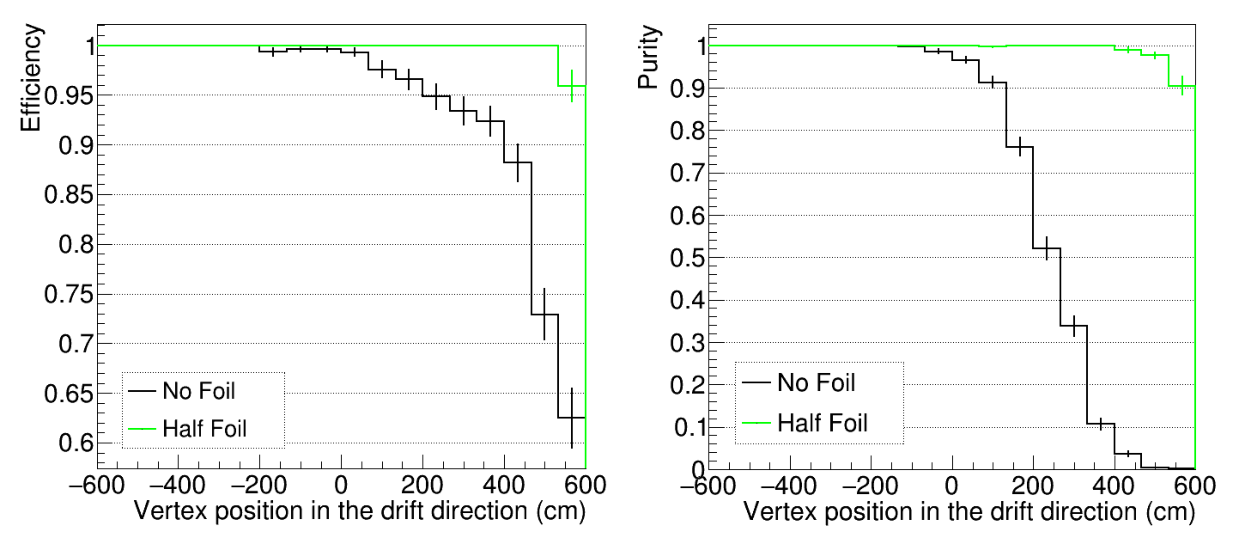
\includegraphics[width=0.90\textwidth]{graphics/dppd_ndk_efficiency.pdf}
    \end{dunefigure}

%%%%%%%%%%%%%%%%%%%%%%%%%%%%%%%%%%%%%%%%%%%%%%%%%%%%%%%%%%%%%%%%%%%%

\subsection{Supernova Burst Triggering}
\label{subsec:dp-pds-performance_trigger}

We have also studied how well the \dword{dp} \dshort{pds} triggers on an \dword{snb} occurring in our galactic neighbourhood. As described in Section~\ref{sec:dp-pds-requirements}, this is one of the primary goals of the \dword{pds}. To this end, \dword{snb} \nue \dword{cc} interactions have been generated with MARLEY \cite{marley} in our baseline \dword{pds} design with reflector/\dword{wls} panel assemblies installed in the top half of the \dword{fc}. In \dword{dune}, a real-time algorithm should provide trigger primitives by searching for \dshort{pmt} hits and optical clusters, where the latter combine several hits together based on their time/spatial information. Compared to the \dword{ndk} case, the reconstructed optical signals are much weaker because the typical deposited energies per \dword{snb} neutrino interaction are approximately \SI{20}{\MeV}. The online clustering process is similar to the offline cluster reconstruction discussed in Section~\ref{subsec:dp-pds-performance_t0}, albeit with some differences related to the lack of trigger information and detailed event reconstruction at this stage:
%
\begin{itemize}
\item Real-time optical clusters must have a minimum hit multiplicity to suppress clusters induced by radiological activity or \dword{pmt} dark counts. The higher the hit multiplicity, the lower the background cluster rate.
\item \dword{pds} spatial information is only used to group hits into separate clusters,  not to match \dword{pds} clusters with \dword{tpc} tracks in the plane perpendicular to the drift as in Section~\ref{subsec:dp-pds-performance_t0}.
\item Real-time optical clusters must be continuously reconstructed, while in Section~\ref{subsec:dp-pds-performance_t0}, only the \SI{7.5}{\milli\s} period preceding a charge-based trigger signal, corresponding to the maximum drift time, is considered.
\end{itemize}
%
In this case, the optimal real-time cluster reconstruction parameters, including a minimum hit multiplicity per cluster requirement, yield a \SI{0.05}{\Hz} radiological background cluster rate for an \dword{snb} \nue \dword{cc} signal cluster efficiency of \SI{11.8}{\%}. Once the optimal cluster parameters are found, the computation of the \dshort{pds}-based \dword{snb} trigger efficiency as a function of \dword{snb} distance is performed as follows:

\begin{itemize}
\item First, the minimum number of reconstructed clusters required in a \SI{2}{\s} time window  to issue a trigger is found\footnote{A \SI{2}{\s} time window was found to be optimal and is assumed throughout this section.}. The minimum cluster multiplicity is set by the requirement of one fake trigger per month at most (see Section~\ref{sec:dp-pds-requirements}) and by the radiological background cluster rate. The higher the background cluster rate, the higher the minimum cluster multiplicity must be to meet the $<$\num{1}/month fake trigger rate requirement. As mentioned above, the clustering optimization procedure yields a background cluster rate of \SI{0.05}{\Hz} or, on average, \num{0.1} clusters per \SI{2}{\s} window. For such a background rate level, a minimum cluster multiplicity of $\ge$\num{3} per \SI{2}{\s} time window is required for a $<$\num{1}/month fake trigger rate.
%
\item Second, and given the cluster parameters and minimum cluster multiplicity defined in the first step, the \dword{snb} triggering efficiency as a function of the number of \dword{snb} interactions is computed. For a \SI{11.8}{\%} average efficiency of reconstructing single \dword{snb} \nue interactions with the \dshort{pds}, and a minimum cluster multiplicity of \num{3} to issue a trigger, approximately \num{3}/\num{0.118}$\simeq$ \num{25} interactions must occur in the \dword{fd} module and within \SI{2}{\s} to obtain a non-negligible trigger efficiency. 
%
\item Third, and finally, the \dword{snb} triggering efficiency as a function of \dword{snb} distance is obtained. We use the theoretical assumptions shown in Figure~\ref{fig:dppd_snbassumptions} to extract the number of \dword{snb} neutrino interactions in a \SI{2}{\s} time window and in one \dword{dp} \dword{fd} module as a function of \dword{snb} distance. The left panel of Figure~\ref{fig:dppd_snbassumptions} shows the time-integrated expected number of \dword{snb} neutrino interactions as a function of distance, while the right panel in Figure~\ref{fig:dppd_snbassumptions} shows the assumed time profile of the burst during the first \SI{10}{\s}. Several hundred \dword{snb} neutrino interactions are expected in one \dword{dp} \dword{fd} module for a \SI{10}{\kilo\parsec} distant \dword{snb}\footnote{It is customary to evaluate the performance of \dword{snb} detectors for a \dword{snb} distance of \SI{10}{\kilo\parsec}, as this is approximately the distance to the Galactic Center.}, and about half of them are expected within the first \SI{2}{\s}. Given our earlier estimate that about \num{25} interactions should be sufficient for a non-negligible trigger efficiency, clearly, the \dshort{pds} should provide high \dword{snb} trigger efficiency for an \dword{snb} at a \SI{10}{\kilo\parsec} distance.
\end{itemize}

\begin{dunefigure}[SN burst triggering assumptions.]{fig:dppd_snbassumptions}
     {Left panel: expected number of \dword{snb} \nue \dshort{cc} interactions in one \dpactivelarmass active mass DP module as a function of \dword{snb} distance. The different green lines indicate different \dword{snb} models. Right panel: expected time profile of the \dword{snb}.}
    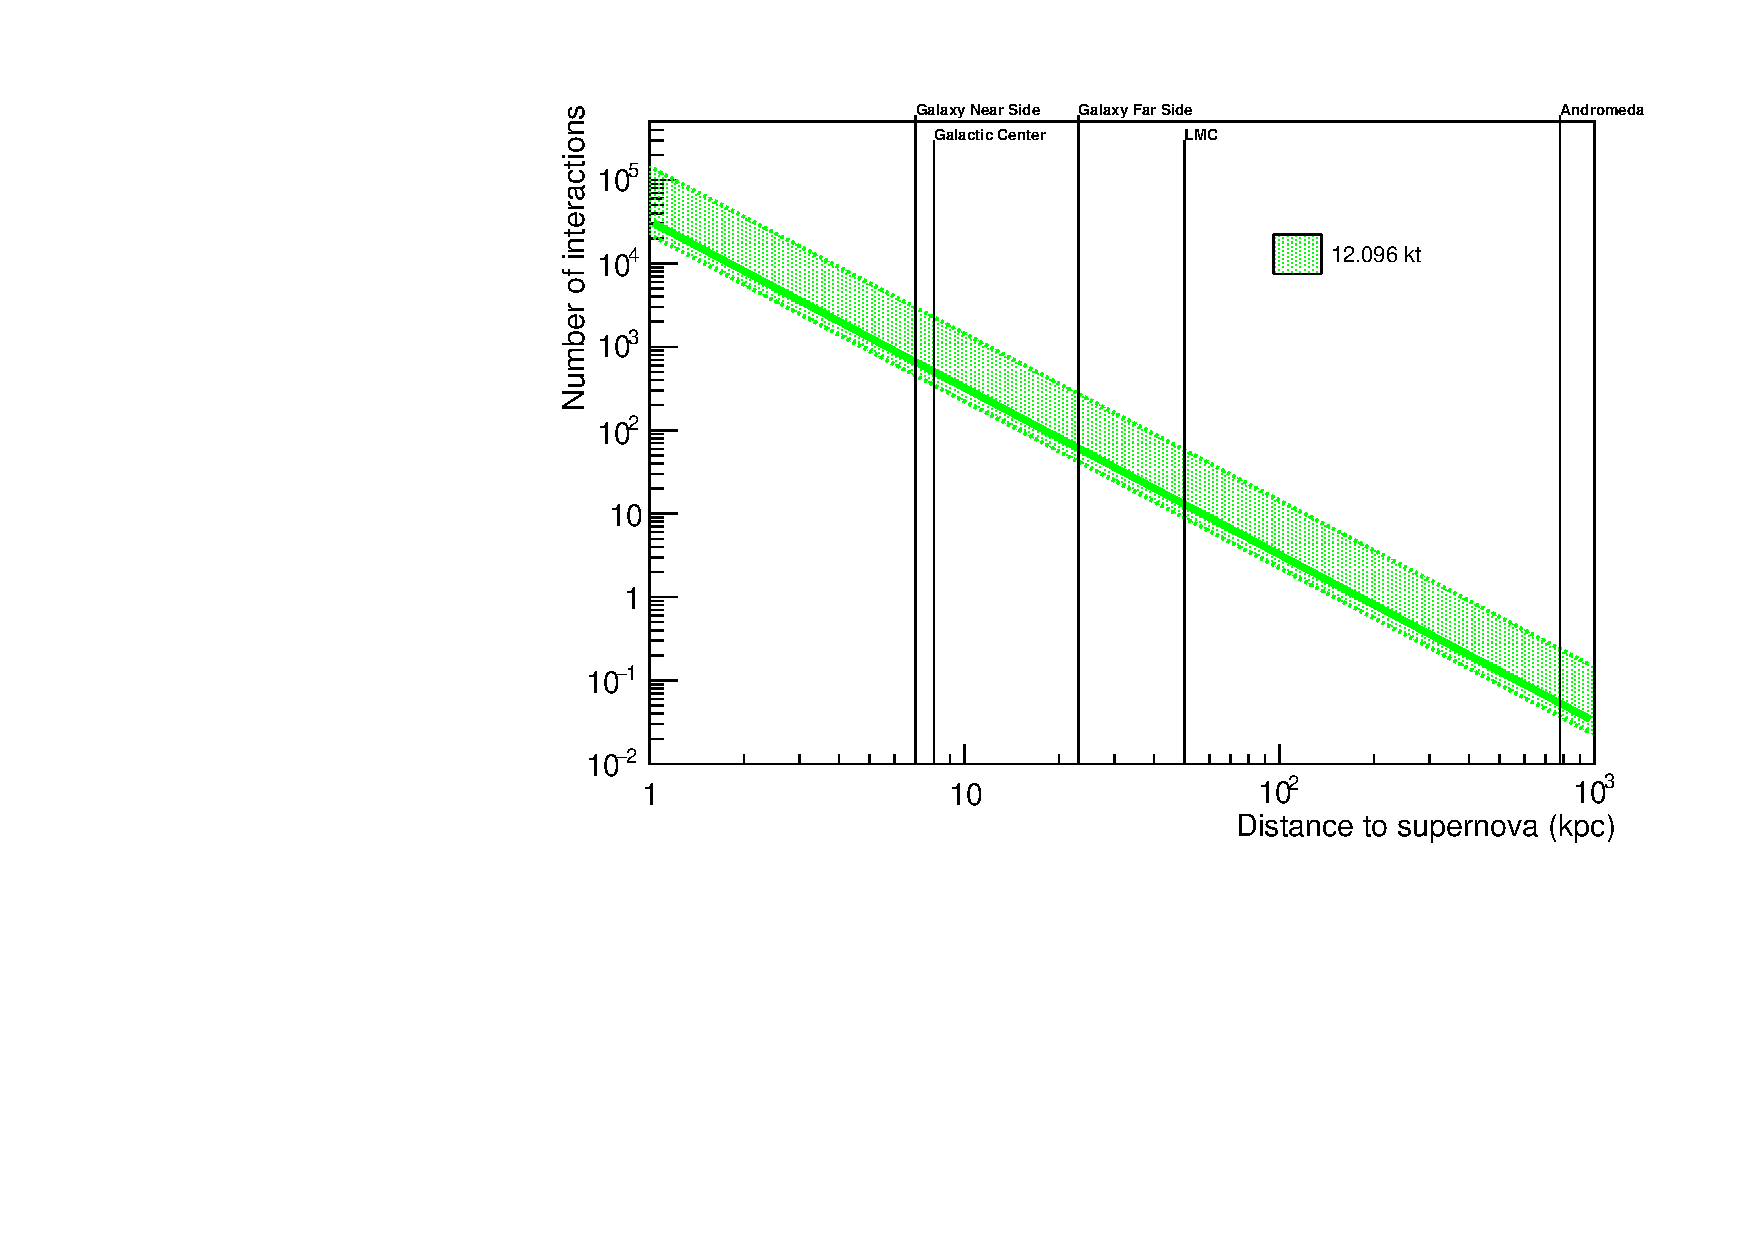
\includegraphics[width=0.49\textwidth]{graphics/dppd_events_vs_sndistance.pdf} \hfill
    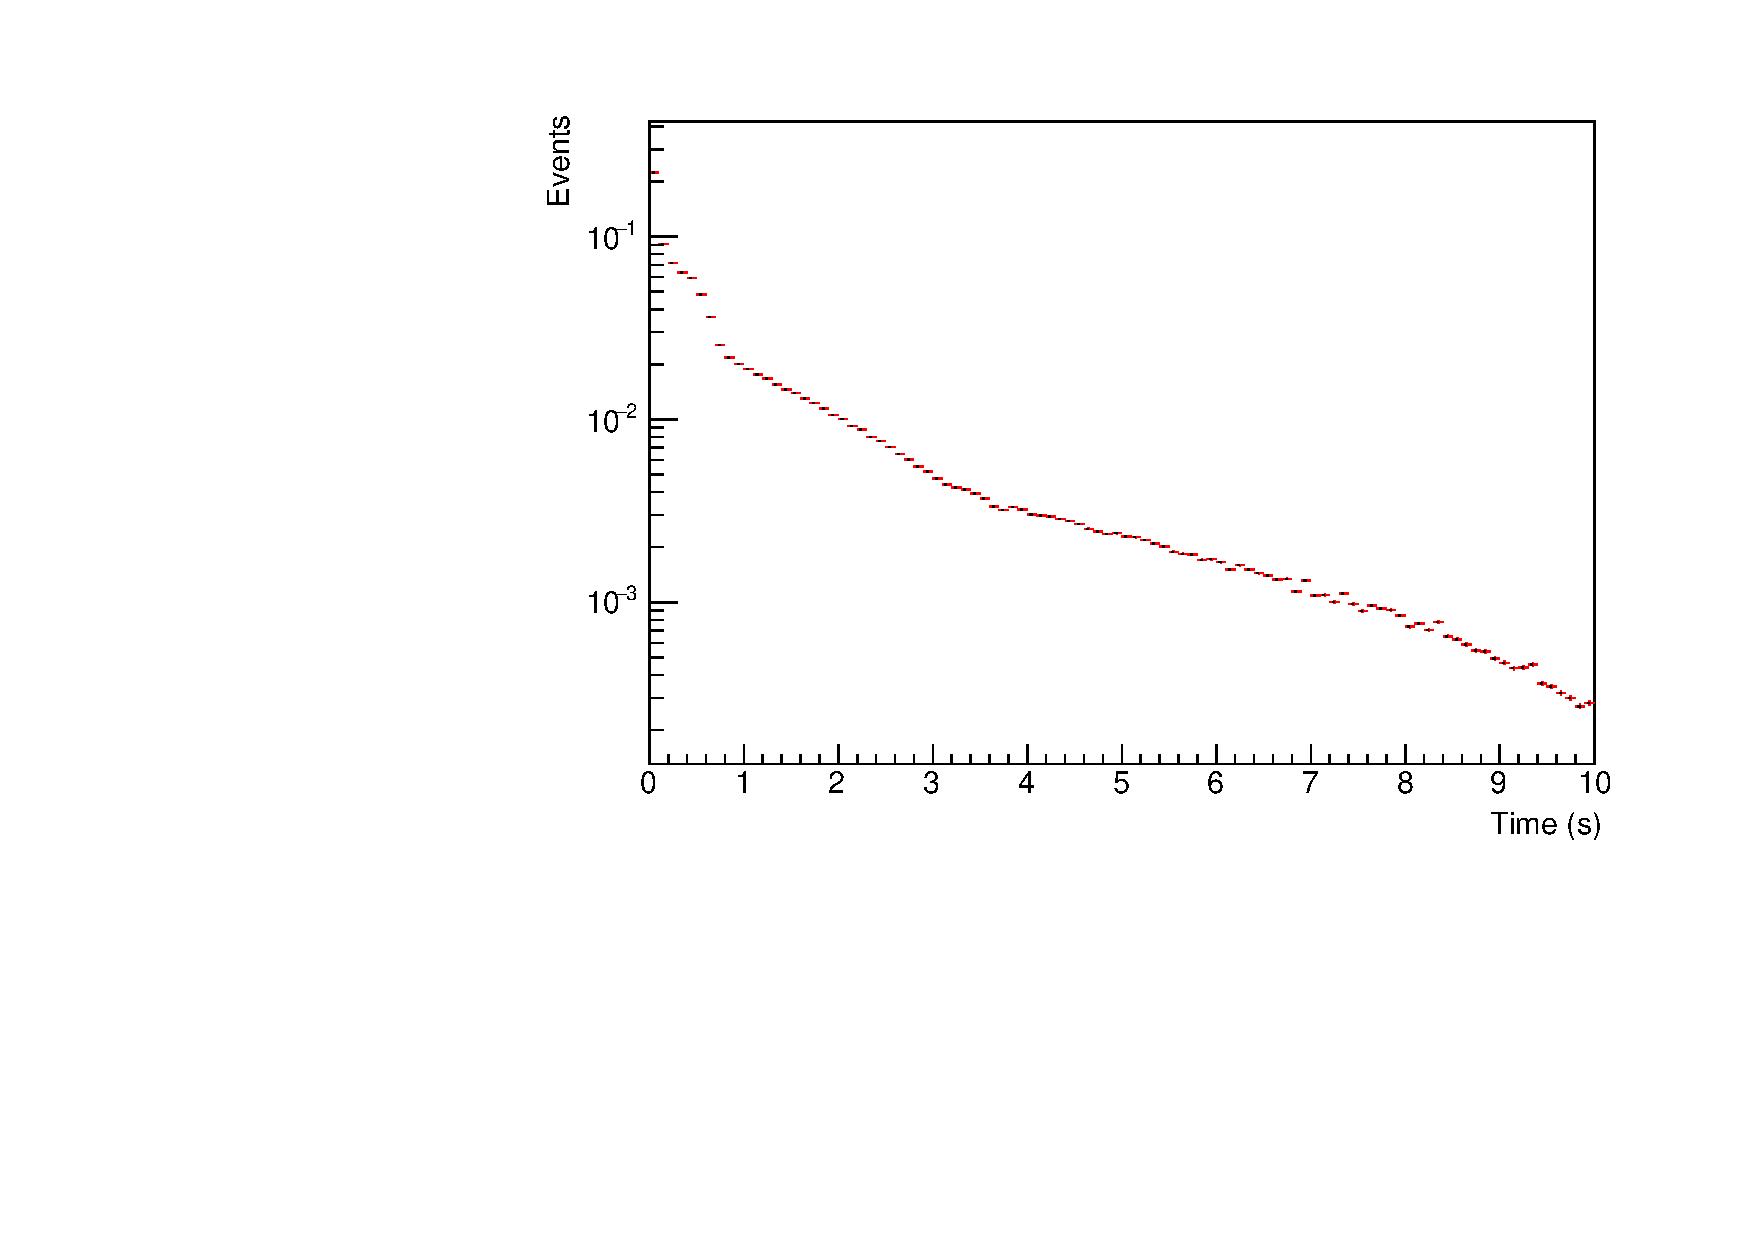
\includegraphics[width=0.49\textwidth]{graphics/dppd_sntime_profile.pdf} 
    \end{dunefigure}

The \dword{snb} triggering efficiency, computed following the procedure described above and as a function of \dword{snb} distance, is shown in Figure~\ref{fig:dppd_snbefficiency_vs_sndistance_half_foils}. The figure shows how the \dword{snb} triggering efficiency is affected by different choices in cluster reconstruction parameters. The best trigger efficiency found for the cluster parameters, yielding the lowest background cluster rate, is \SI{0.05}{\Hz}. In this case, a trigger efficiency in excess of \num{90}\% is obtained up to \dword{snb} distances of approximately \SI{25}{\kilo\parsec}. Therefore, the \dshort{pds} should yield a highly efficient trigger for \dword{snb} occurring anywhere in the Milky Way. 

\begin{dunefigure}[\dword{snb} triggering efficiency for different cluster reconstruction parameters.]{fig:dppd_snbefficiency_vs_sndistance_half_foils}
     {\dword{snb} triggering efficiency using \dword{dp} \dshort{pds} information as a function of \dword{snb} distance. Different curves indicate different choices of the optical cluster reconstruction parameters, resulting in different \dword{snb} \nue signal detection efficiencies (DE) and radiological background rates (BGR).}
    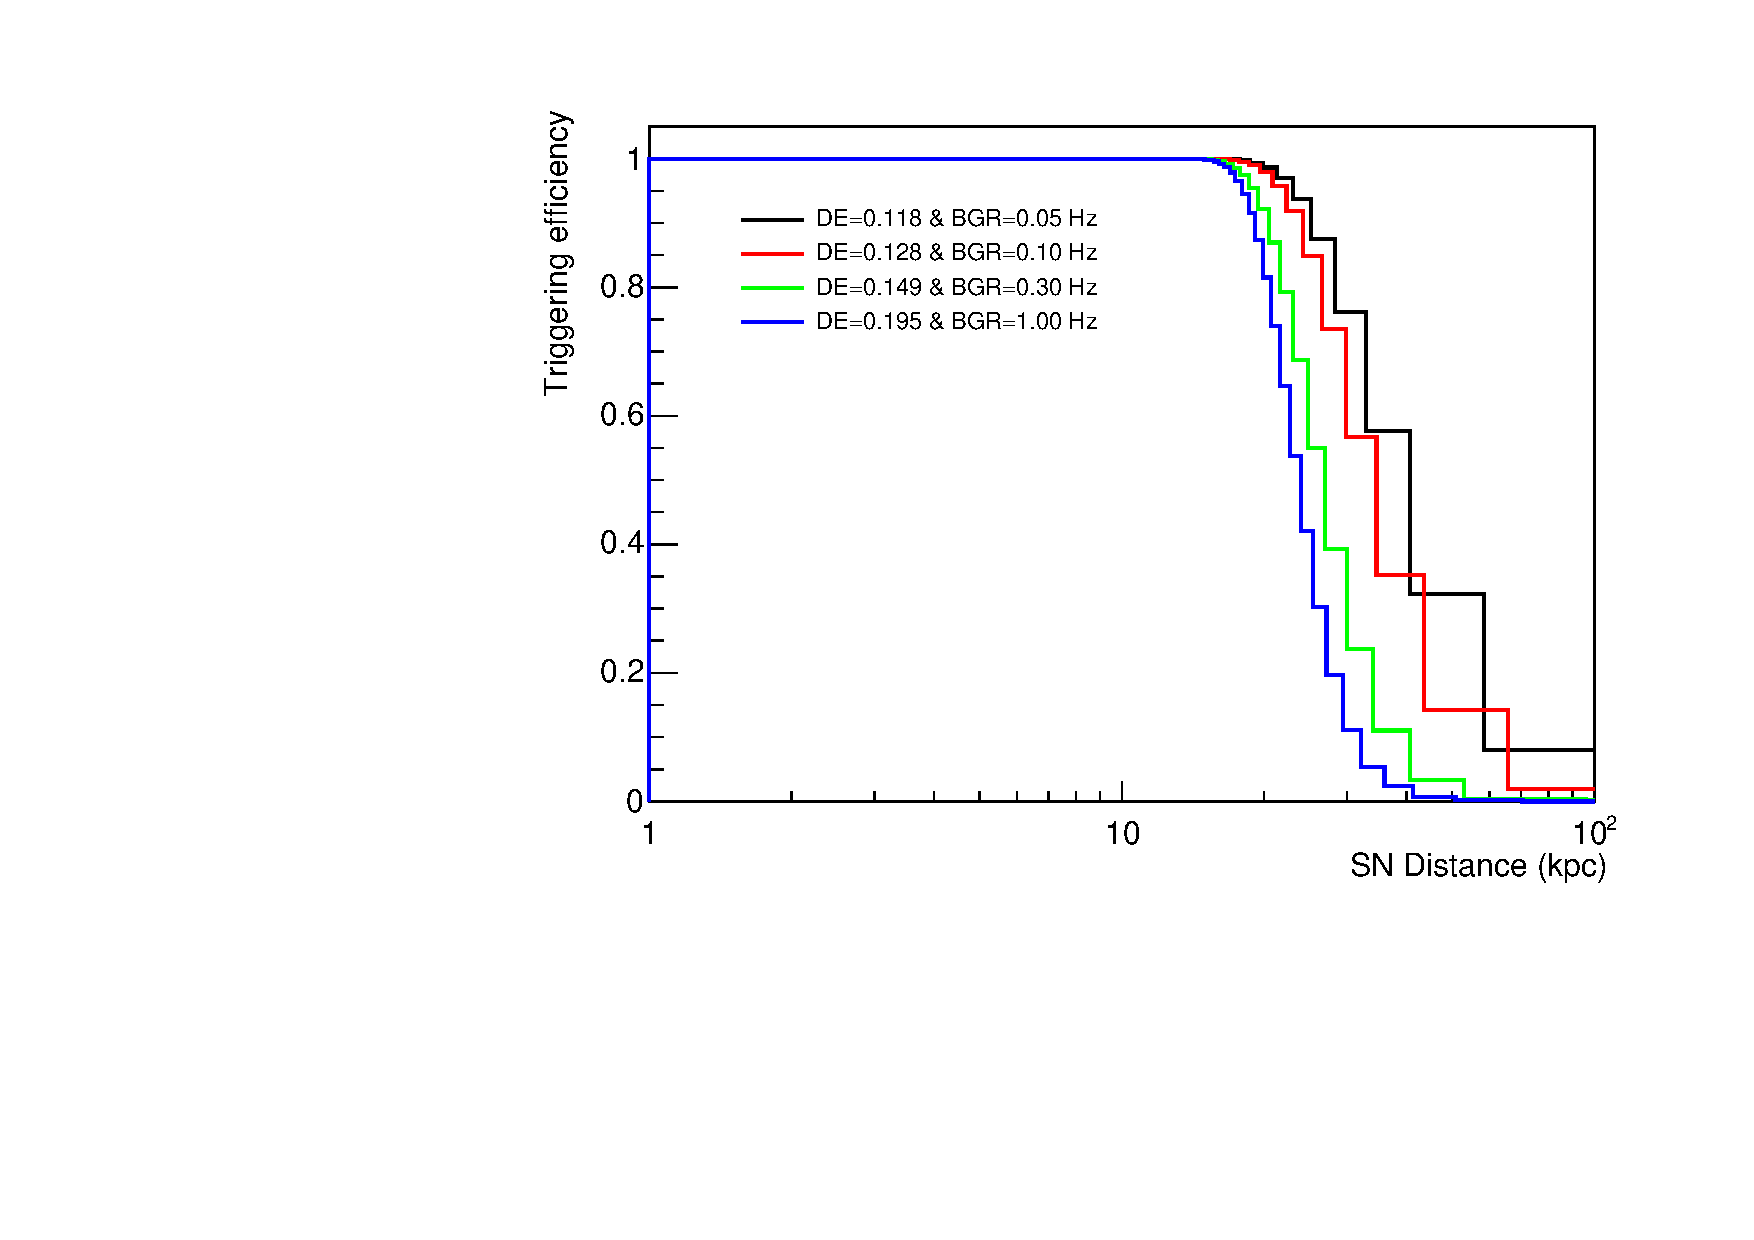
\includegraphics[width=0.6\textwidth]{graphics/dppd_snbefficiency_vs_sndistance_half_foils.pdf}
    \end{dunefigure}

Figure~\ref{fig:dppd_snbefficiency_vs_sndistance_comparison} shows how the \dword{snb} trigger efficiency of the baseline configuration with \dword{wls} reflector foils along the upper \dword{fc} half compares with alternative choices, namely no foils and full foils. Our minimum \dword{snb} trigger efficiency requirement of \num{90}\% at \SI{20}{\kilo\parsec} (see Sec.~\ref{subsec:dp-pds-requirements_requirements}) should be (barely) reachable even for the no foil configuration. In this case, the average light yield is expected to be about \SI{5}{PEs/MeV}, see Table~\ref{tab:dp-pds-light-yields}. For this reason, Table~\ref{tab:specs:just:DP-PDS} quotes \SI{>5}{\dwords{pe}/\MeV} as the average light yield requirement. On the other hand, the results improve noticeably with increased foil coverage, as $>$\num{90}\% trigger efficiency extends to approximately \num{25} and \SI{36}{\kilo\parsec} for the half foil and full foil configurations, respectively. 

\begin{dunefigure}[\dword{snb} triggering efficiency for different \dword{wls} foil configurations.]{fig:dppd_snbefficiency_vs_sndistance_comparison}
     {\dword{snb} triggering efficiency as a function of \dword{snb} distance for three different \dword{wls} foil configurations.}
    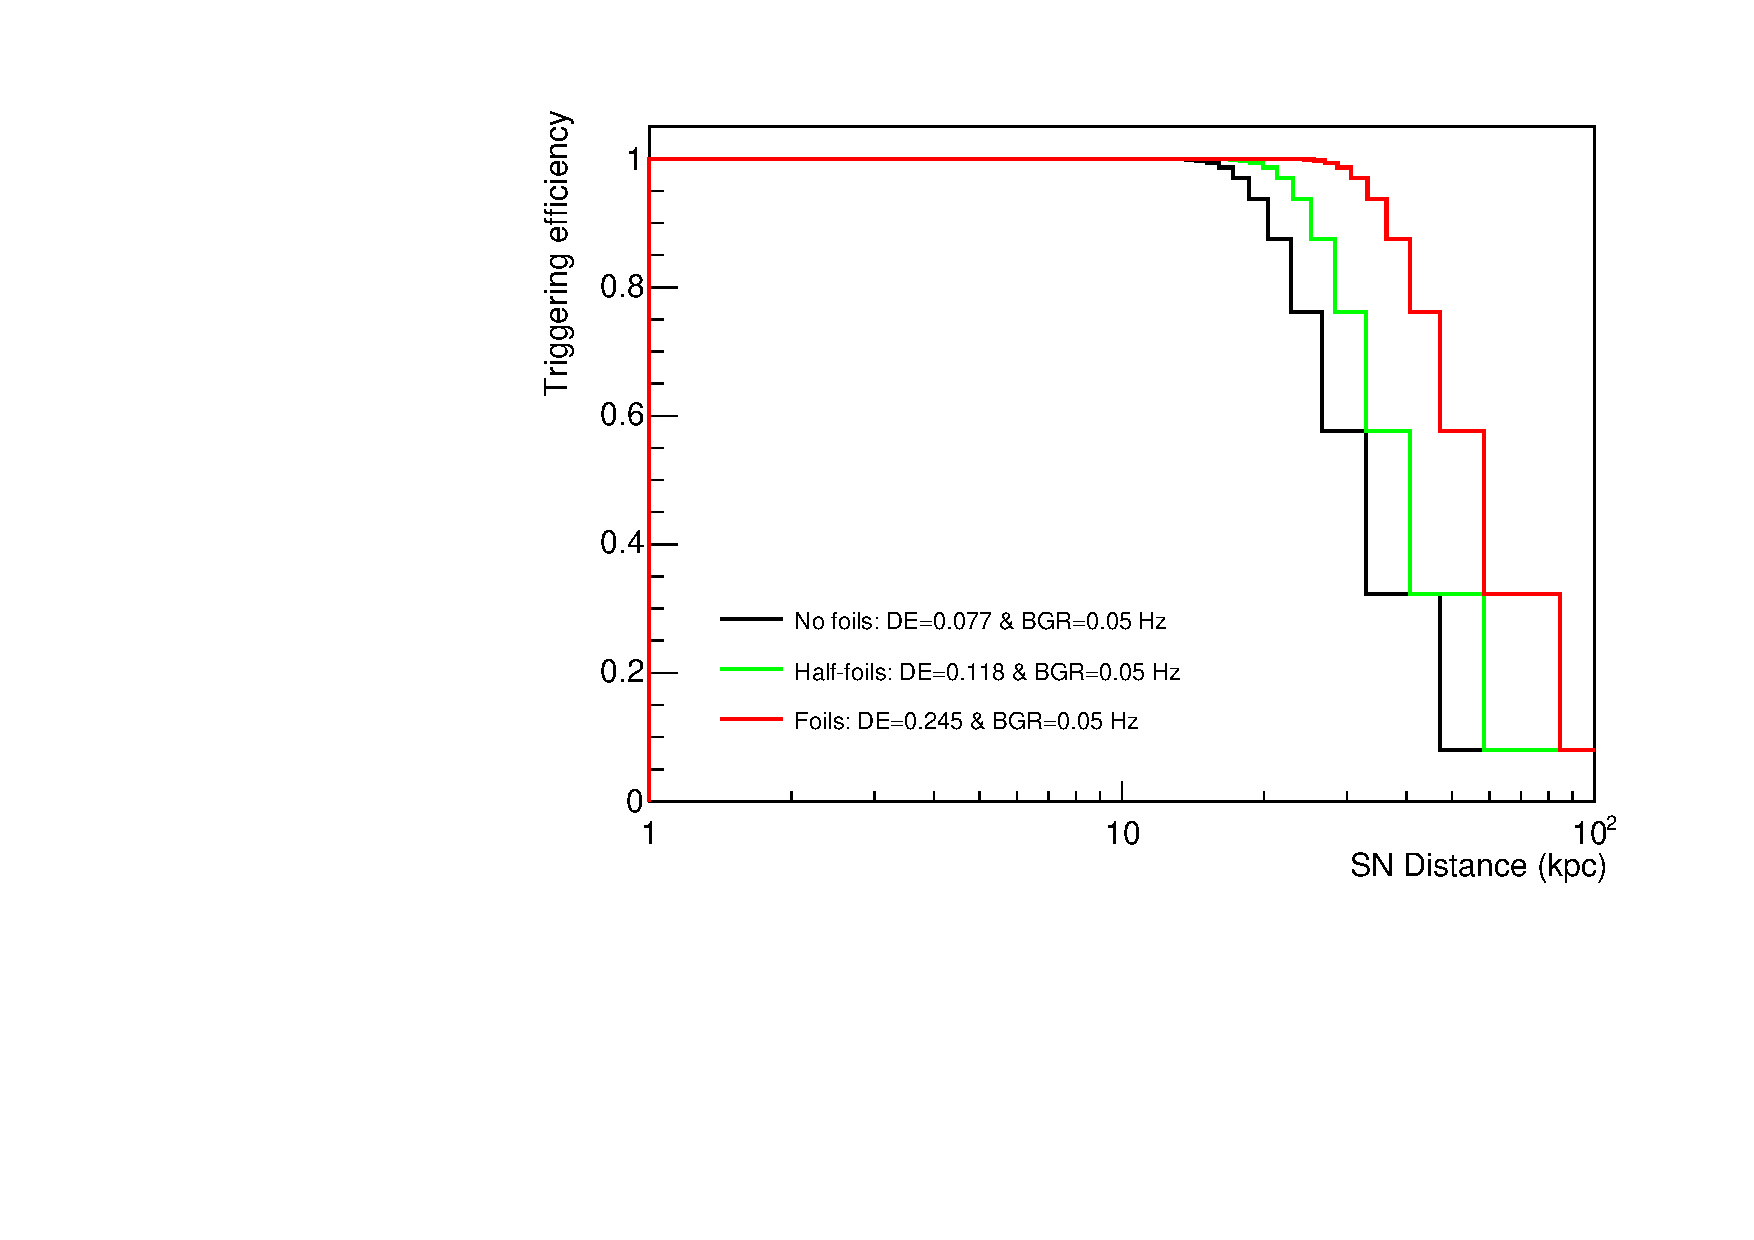
\includegraphics[width=0.6\textwidth]{graphics/dppd_snbefficiency_vs_sndistance_comparison.pdf}
    \end{dunefigure}

%%%%%%%%%%%%%%%%%%%%%%%%%%%%%%%%%%%%%%%%%%%%%%%%%%%%%%%%%%%%%%%%%%%%

\subsection{Event Energy Reconstruction}
\label{subsec:dp-pds-performance_calorimetry}

In addition to timing and triggering information, the \dword{pds} can also provide event energy information via the intensity of the reconstructed optical flashes. We focus in this section on beam neutrino interactions generated via the \dshort{genie} event generator \cite{Andreopoulos:2009rq}, as described in Section~\ref{subsec:dp-pds-requirements_requirements}.

A first requirement for a competitive energy reconstruction performance with the \dword{pds} is that optical hit saturation effects are kept to a manageable level by the \dword{pds} and associated readout electronics. Figure~\ref{fig:dppd_saturation} shows the expected average hit charge and average hit amplitude as a function of drift position of the neutrino interaction vertex for \SI{3}{\GeV} beam \nue \dshort{cc} interactions. For each event, the average is computed by considering hit \dshort{pds} channels only, that is, \dwords{pmt} detecting a charge of at least \SI{1}{PE}. The average hit charge per event is approximately \SIrange{50}{300}{} for \SI{3}{\GeV} beam \nue \dshort{cc} interactions throughout the \dword{tpc} active volume. The average charge is expressed in \dwords{pe}, with the average amplitude in \dwords{pe} per \SI{4}{\nano\s} time bin. This time bin width is comparable with the \SI{6}{\nano\s} timescale characteristic of the prompt scintillation light in \dshort{lar}. For events near the cathode plane, about \SI{300}{\dwords{pe}} per hit channel are detected, corresponding to a maximum amplitude over \SI{4}{\nano\s} of about \SI{50}{\dwords{pe}}. The factor of 6 difference between average charge and average amplitude is because only \SI{23}{\%} of the scintillation light is prompt and (to a smaller extent) because of additional time smearing introduced by light propagation to the same \dword{pmt} from different \dshort{lar} voxels containing energy deposits. From these plots, we conclude that the \dshort{pds} signal readout should withstand signal amplitudes of at least \SI{100}{\dwords{pe}} over \SI{6}{\nano\s} to mitigate saturation effects (see Table~\ref{tab:specs:just:DP-PDS}).

\begin{dunefigure}[Average charge and amplitude per hit channel in beam neutrino interactions.]{fig:dppd_saturation}
{Expected average hit charge (left panel, in \dwords{pe}) and average hit amplitude (right panel, in \dwords{pe} per \SI{4}{\nano\s} time bin) as a function of event drift position for \SI{3}{\GeV} beam \nue \dshort{cc} interactions. The scatter plots  contain one entry per event, and the average is for hit \dshort{pds} channels only.}
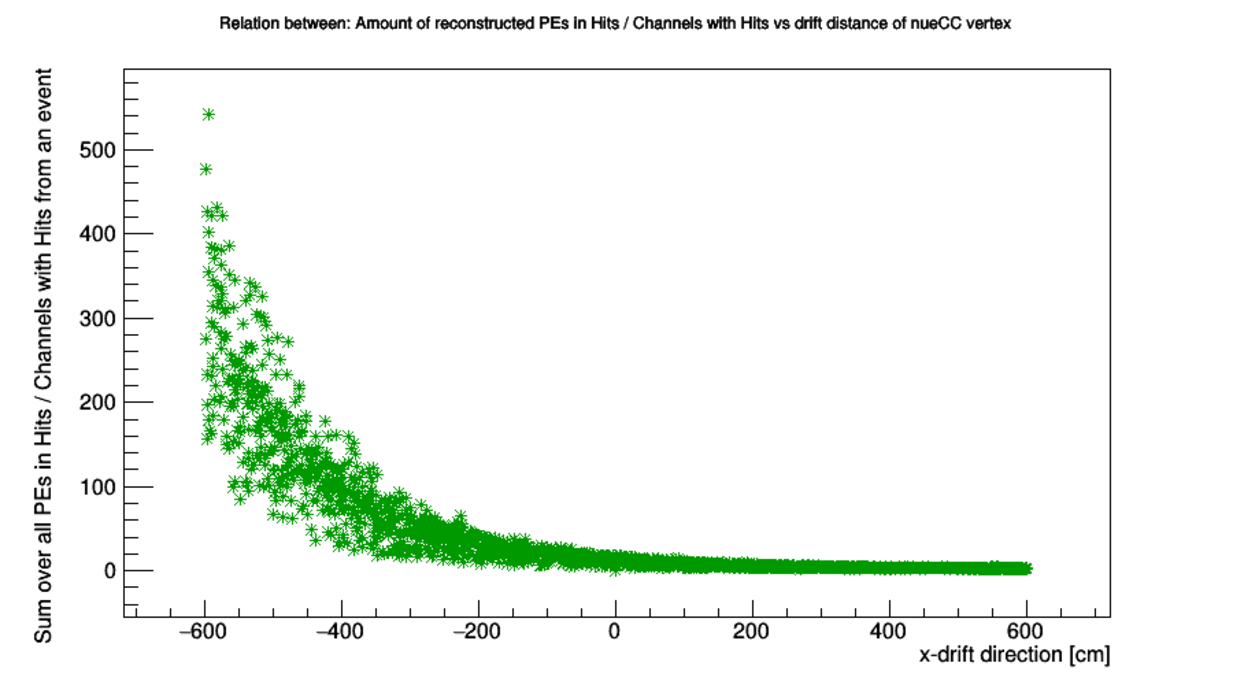
\includegraphics[trim={0cm 0cm 0cm 1.cm}, clip, width=0.49\textwidth]{graphics/dppd_avg_charge_per_channel.pdf} \hfill
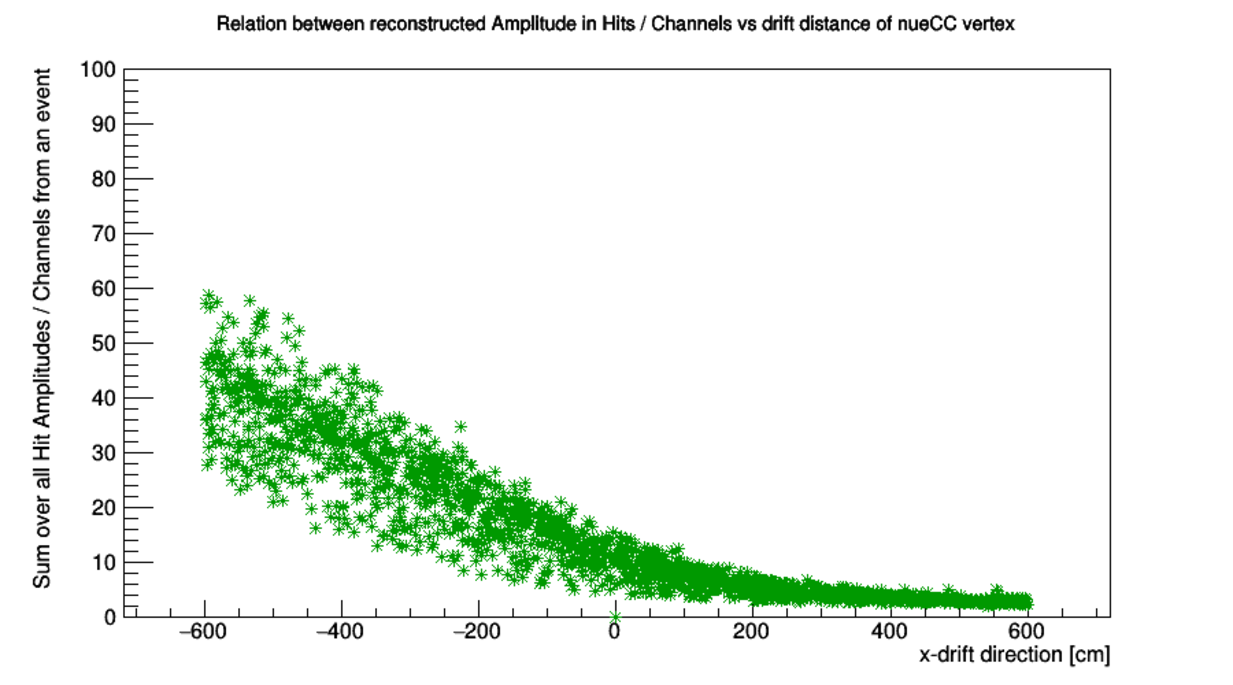
\includegraphics[trim={0cm 0cm 0cm 1.cm}, clip, width=0.49\textwidth]{graphics/dppd_avg_amplitude_per_channel.pdf}
\end{dunefigure}

The neutrino energy for the same \SI{3}{\GeV} beam \nue \dshort{cc} interactions has been reconstructed using \dword{pds} information as follows:
%
\begin{equation}
\label{eq:dppd_ereco} 
%    E_{\rm reco} = \frac{Q}{\varepsilon_{\rm \dword{pmt}}\cdot %V_{\dword{pds}}(\vec{x}_{\rm int})\cdot Y}
E_{\rm reco} = \frac{Q}{\varepsilon_{\rm PMT}\cdot V_{PDS}(\vec{x}_{\rm int})\cdot Y}
\end{equation}
%
\noindent where $Q$ is the total charge (in \dwords{pe}) of all \dword{pmt} hits reconstructed in the event, $\varepsilon_{\rm PMT}$ is the \dword{pmt} quantum efficiency, $V_{PDS}(\vec{x}_{\rm int})$ is the \dword{pds} visibility at the neutrino interaction vertex $\vec{x}_{\rm int}$, defined as the fraction of \lar scintillation photons that reach one of the \dword{pmt} photo-cathode surfaces, $Y=\SI{2.4e4}{photons/MeV}$ is the scintillation light yield, and $E_{\rm reco}$ is the resulting reconstructed energy. In Eq.~\ref{eq:dppd_ereco}, we include \dword{pmt} dark counts in time coincidence with the beam, and we assume that \dword{tpc} information will provide the neutrino interaction vertex information that is needed for the visibility estimate. The event energy reconstructed in this way is shown in the right panel of Fig.~\ref{fig:dppd_beam_calorimetry}, for a sample of neutrino interactions occurring in the \lar fiducial volume. The distribution peaks at about \SI{2.2}{GeV}, somewhat lower than the generated neutrino energy of \SI{3}{GeV}. A gaussian fit to this distribution yields about a \num{20}\% resolution. This value meets the requirement described in Sec.~\ref{subsec:dp-pds-requirements_requirements}, and confirms that the \dword{pds} should be able to provide energy information that is competitive with the \dune \dword{tpc}. Figure~\ref{subsec:dp-pds-requirements_requirements} also shows, in the left panel, the true deposited energy $E_{\rm depo}$ in the \lar active volume for the same simulated events. This distribution shows how an ideal detector could reconstruct event energy, for beam neutrino events. From the comparison of $E_{\rm depo}$ and $E_{\rm reco}$, we conclude that a significant portion of the bias and smearing seen in $E_{\rm reco}$ is already present at the $E_{\rm depo}$ level, and hence cannot be corrected for in a model-independent way. Figure~\ref{fig:dppd_beam_calorimetry2} shows that $E_{\rm reco}$ and $E_{\rm depo}$ are highly correlated, as expected. 

\begin{dunefigure}[Deposited energy and \dword{pds}-reconstructed energy for beam neutrino interactions.]{fig:dppd_beam_calorimetry}
{Expected deposited energy in \lar (left panel) and \dword{pds}-reconstructed energy (right panel) for \SI{3}{\GeV} beam \nue \dshort{cc} interactions in the \lar fiducial volume. A gaussian fit is superimposed to the reconstructed energy distribution.}
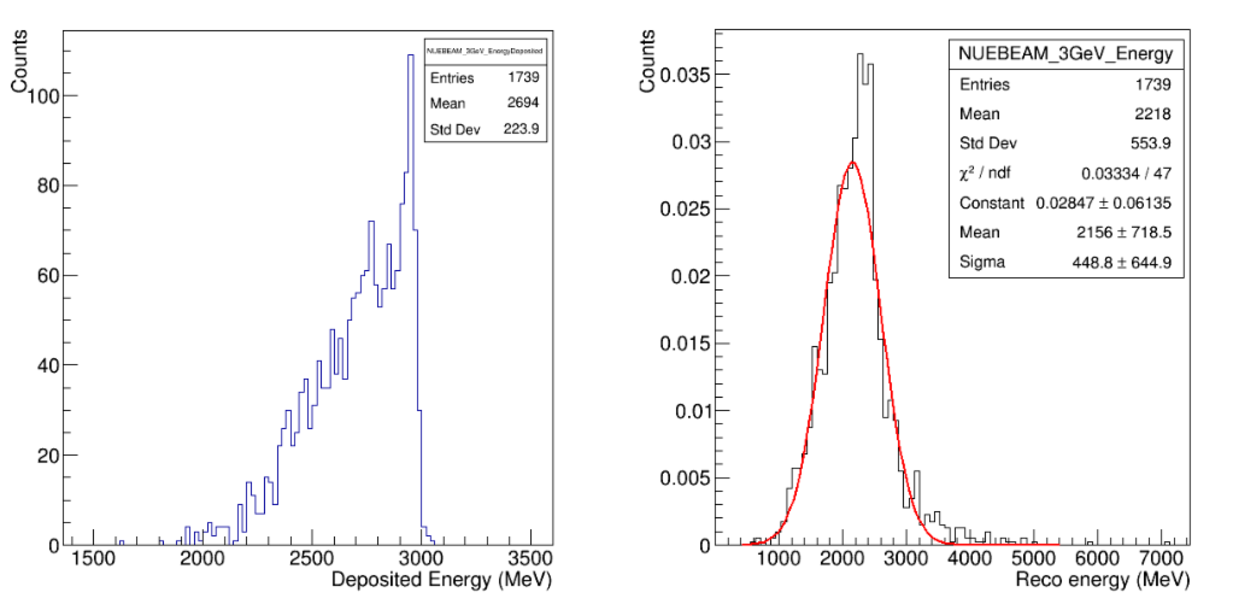
\includegraphics[width=0.95\textwidth]{graphics/dppd_beam_calorimetry.pdf} 
\end{dunefigure}

\begin{dunefigure}[Correlation between \dword{pds}-reconstructed energy and deposited energy for beam neutrino interactions.]{fig:dppd_beam_calorimetry2}
{Correlation between \dword{pds}-reconstructed energy (vertical axis) and true deposited energy in \lar (horizontal axis) for \SI{3}{\GeV} beam \nue \dshort{cc} interactions in the \lar fiducial volume.}
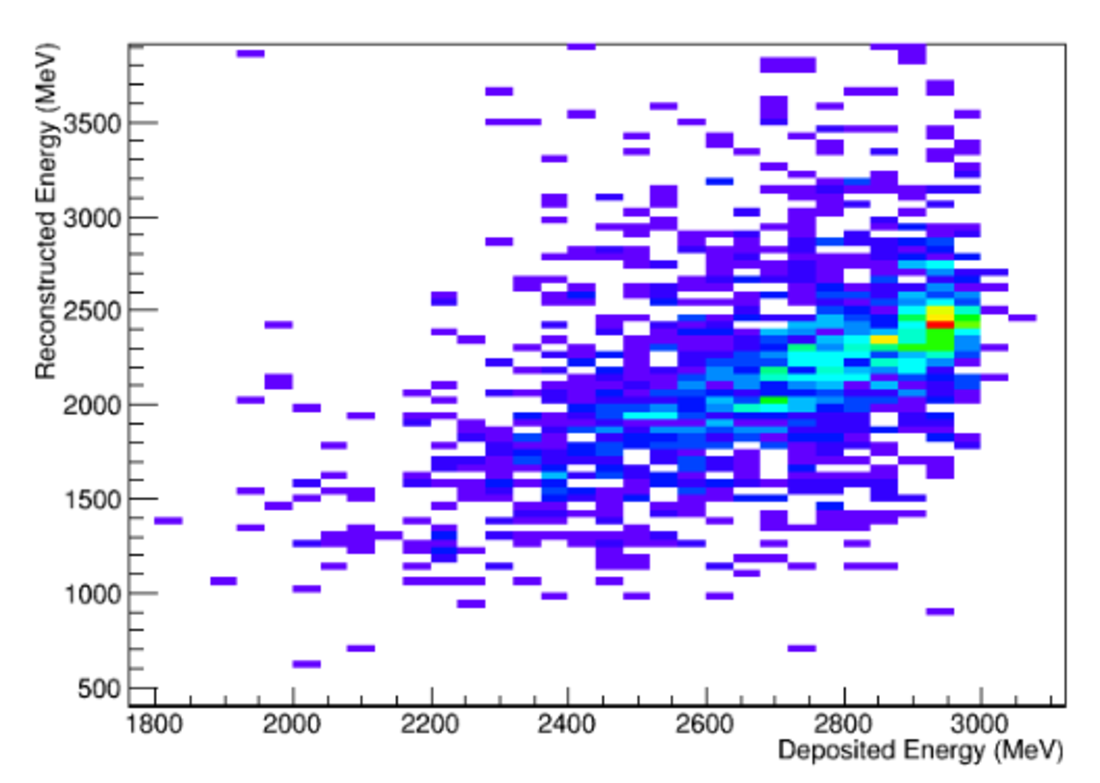
\includegraphics[width=0.60\textwidth]{graphics/dppd_beam_calorimetry2.pdf} 
\end{dunefigure}

We expect to improve the energy resolution performance shown above in two ways:
\begin{description}
   \item[Improved \dword{pds} design:] the results shown above were obtained for the no \dword{wls} foil detector configuration. Studies for the baseline half foil configuration are ongoing. Because of the more uniform response of the baseline design, we expect that the energy resolution will improve.  
   \item[Improved energy reconstruction algorithm:] Eq.~\ref{eq:dppd_ereco} assumes that all the energy is deposited at the neutrino vertex. In practice, events have a certain spatial extent and energy deposition pattern, which the \dword{tpc} can accurately measure. A reconstruction algorithm that accounts for the event extent is expected to perform better, and is under development.
\end{description}
 